% ===================================================================================================
\chapter{Theory}
% ===================================================================================================

% ---------------------------------------------------------------------------------------------------
\section{Magnetic Confinement Fusion}
% ---------------------------------------------------------------------------------------------------
At a subatomic level, nuclear fusion is governed by two separate fundamental interactions -- the electromagnetic force, which causes the positively charged positrons of two nuclei to repel each other, and the residual strong force, which binds together protons and neutrons to form nuclei. 
Due to their small size and the low number of protons, nuclei of elements lighter than nickel and iron can overcome the electromagnetic repulsion barrier and fuse into a single nucleus, releasing typically orders of magnitude more energy than any process involving chemical bonds.

Since the nuclei have to be brought to within around $10^{-15}$ m from each other in order for the short-ranged strong interaction to outweigh the electromagnetic repulsion, the process of forcing together even the lightest nuclei requires substantial amounts of energy.  
At the cores of stars, the immense pressure combined with temperatures of the order of $10^6$ K brings hydrogen atoms close enough for some of them to cross the repulsion barrier through the quantum mechanical effect of tunnelling \cite{clayton1983principles}.
Without the gravitational mass of a star compressing the fusion fuel, however, we have to rely on various 'dirty tricks' to achieve conditions suitable for a self-sustaining fusion reaction. 
The most promising of these tricks, Magnetic Confinement Fusion (MCF) (in contrast to gravitational confinement occurring in stars) exploits the fact that charged particles can be manipulated using magnetic fields. 
The fuel is heated to temperatures of the order of $10^7$ K, at which point the electrons and nuclei of the fuel atoms will have separated, transitioning into plasma. 
The goal of current MCF projects is to be able to control the plasma using strong magnets, confining it to a limited volume and preventing it from contacting the reactor walls.
The combination of extreme heat and confinement provides an environment suitable for fusion to occur.

Research focusing on MCF has been conducted the early 1950s, with multiple reactor designs, such as the stellarator, Z-pinch and levitated dipole having been proposed throughout the years. 
The tokamak, currently seen as the most promising design for an MCF reactor, was initially developed and first constructed in the late 1950s by Soviet physicists \cite{tokamakorigins}. 
The reactor type is best described by its name, which is a Russian acronym for a "toroidal chamber with magnetic coils" (fig. \ref{fig:tokamak}).

\begin{figure}[!ht]
\center
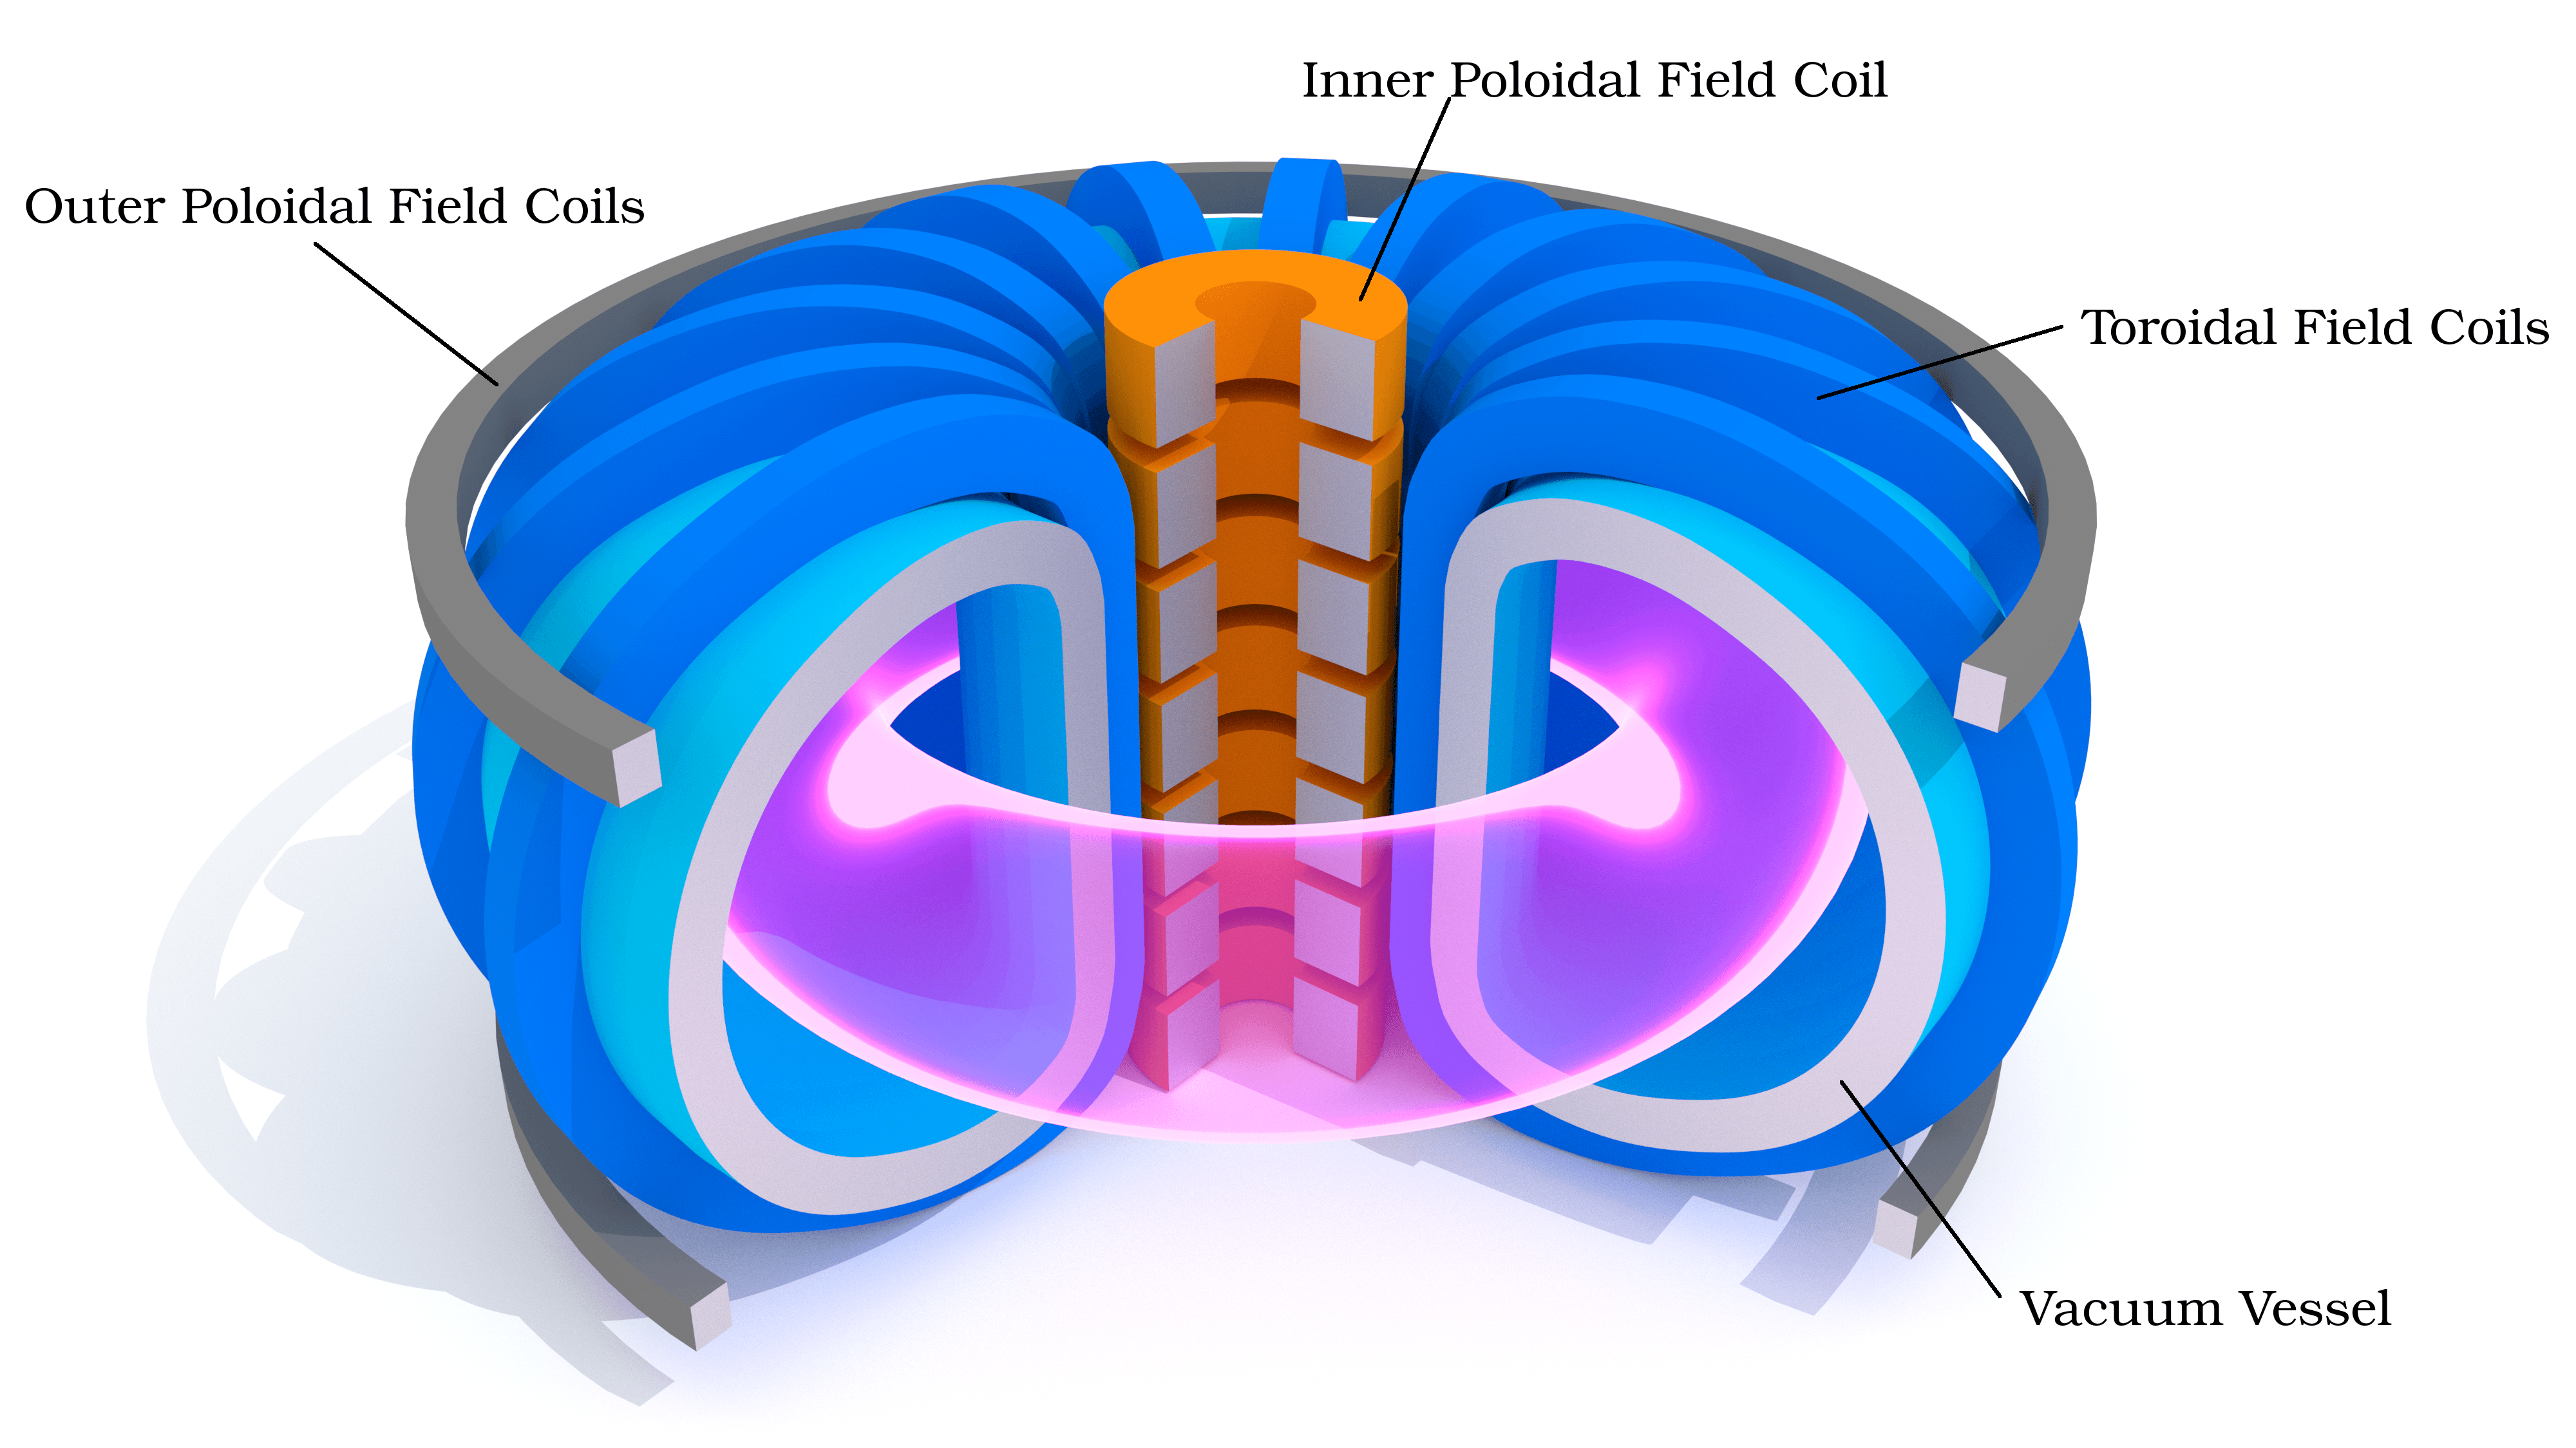
\includegraphics[width=0.8\linewidth]{Schematic-of-a-tokamak.png}
\caption{A schematic view of a tokamak-type fusion reactor.} 
\label{fig:tokamak}
\end{figure}

In principle, any two light enough elements can be fused. 
However, from an fuel-economical point of view, the deuterium-tritium reaction 
\begin{align}
^2_1\rm{H} ~+~ ^3_1\rm{H} ~\rightarrow~ ^4_2\rm{He} ~+~ ^1_0\rm{n} ~+~ 17.58 ~\rm{MeV}
\label{Eq:D-T-reaction}
\end{align}
can be considered one of the most favourable. 
Deuterium can be refined easily out of hydrogen extracted from seawater, while tritium can be produced through transmutation from lithium
\begin{align}
^6_3\rm{Li} ~+~ ^1_0\rm{n} ~\rightarrow~ ^4_2\rm{He} ~+~ ^3_2\rm{H} ~+~ 4.80  ~\rm{MeV}
\end{align}
using the neutrons released from either a fission or fusion reactor, potentially using specific tritium "breeding" structures on the inner surfaces of a tokamak \cite{giancarli2012overview}.


% ---------------------------------------------------------------------------------------------------
\section{Plasma Facing Components in Modern Tokamaks}
% ---------------------------------------------------------------------------------------------------

The extreme conditions contained within a fusion reactor impose strict requirements on the construction materials. 
Energetic neutrons and ions are constantly bombarding the plasma-facing components, causing heating of the reactor vessel and erosion of the walls, potentially hindering the fusion process by contaminating the plasma with heavier atoms. 
In order to protect the vacuum vessel from the intense heat and the erosive effects of plasma particles, the inner walls are covered with a cooled and armoured \textit{blanket}. 
In reactors such as the ITER or the Joint European Torus (JET), the blanket is often covered with beryllium \cite{raffray2012overview}, chosen due to its superior plasma contamination properties.

Located usually at the top or bottom of a tokamak, the \textit{divertor} is a device used for online removal of fusion products and impurities from the plasma.
Positioned at a intersection of magnetic field lines, the plasma-facing surfaces of the divertor are subject to even more extreme particle bombardment than those of the blanket.
For instance, the vertical targets of the ITER divertor, visible in fig. \ref{fig:ITERslice}, are expected to receive heat fluxes of up to 20 MW/m$^2$ \cite{Iter1234Divertor}. 

\begin{figure}[!ht]
\center
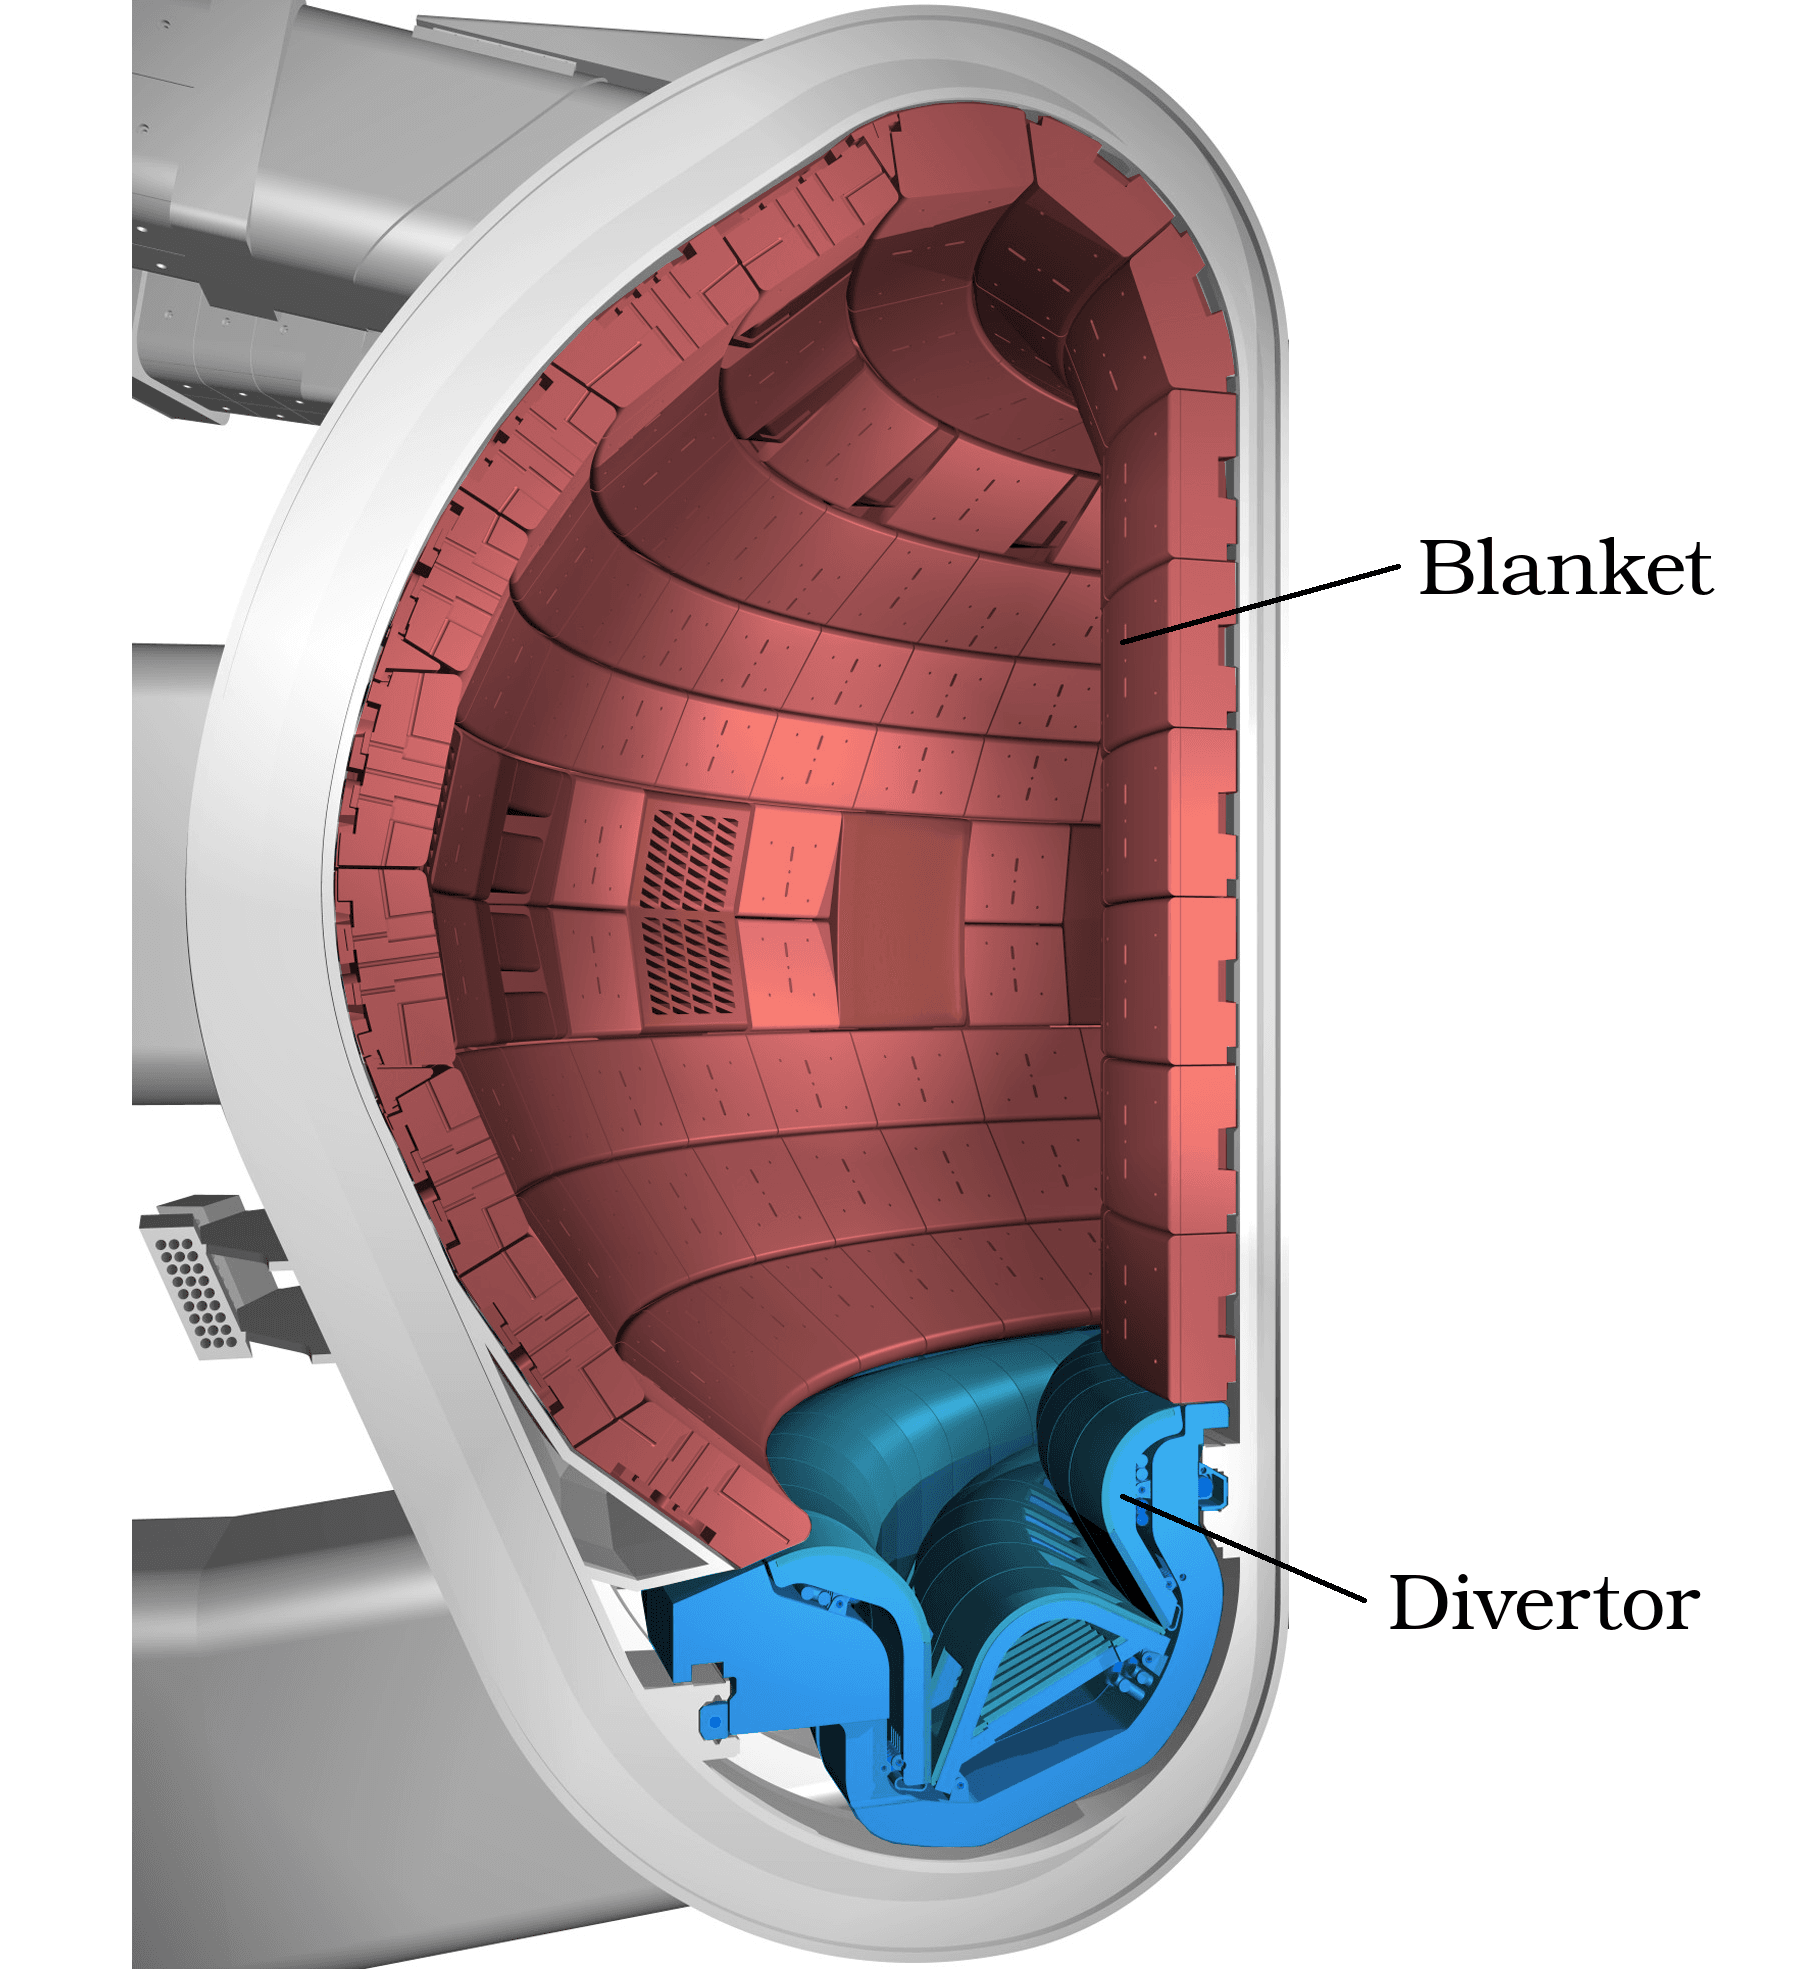
\includegraphics[scale=0.1]{vacuumvessel_edited.png}
\caption{A section of the ITER tokamak with the plasma facing components highlighted. Adapted from http://www.iter.org/, \copyright~ITER Organization}
\label{fig:ITERslice}
\end{figure}

% ---------------------------------------------------------------------------------------------------
\section{Hydrogen Retention in Tungsten}
% ---------------------------------------------------------------------------------------------------
The armour material of choice for the divertor at ITER is tungsten (W) \cite{PITTS2013S48}.
The metal, named after the Swedish word for "heavy stone", is recognized for having the highest melting point of all metals and a hardness superior to that of most steels. 
In its structurally most stable form, W has a body-centered-cubic (BCC) crystal structure, with a lattice constant $a$ of 3.165 \AA.
The equilibrium position for hydrogen in perfect W lattice is at the tetrahedral interstitial position (TIS), shown as black dots in fig. \ref{Fig:bcc}. 

At temperatures $T > 0$ K, any real crystalline materials will contain some amount of crystallographic defects, the most common which are visualized in fig. \ref{Fig:defect_types}. 
The number of these defects increases with the temperature and as the result of irradiation. 
Defects, being disruptions in the periodicity of a lattice, cause an increase in the potential energy of the atomic system. 
\begin{figure}[!ht]
\center
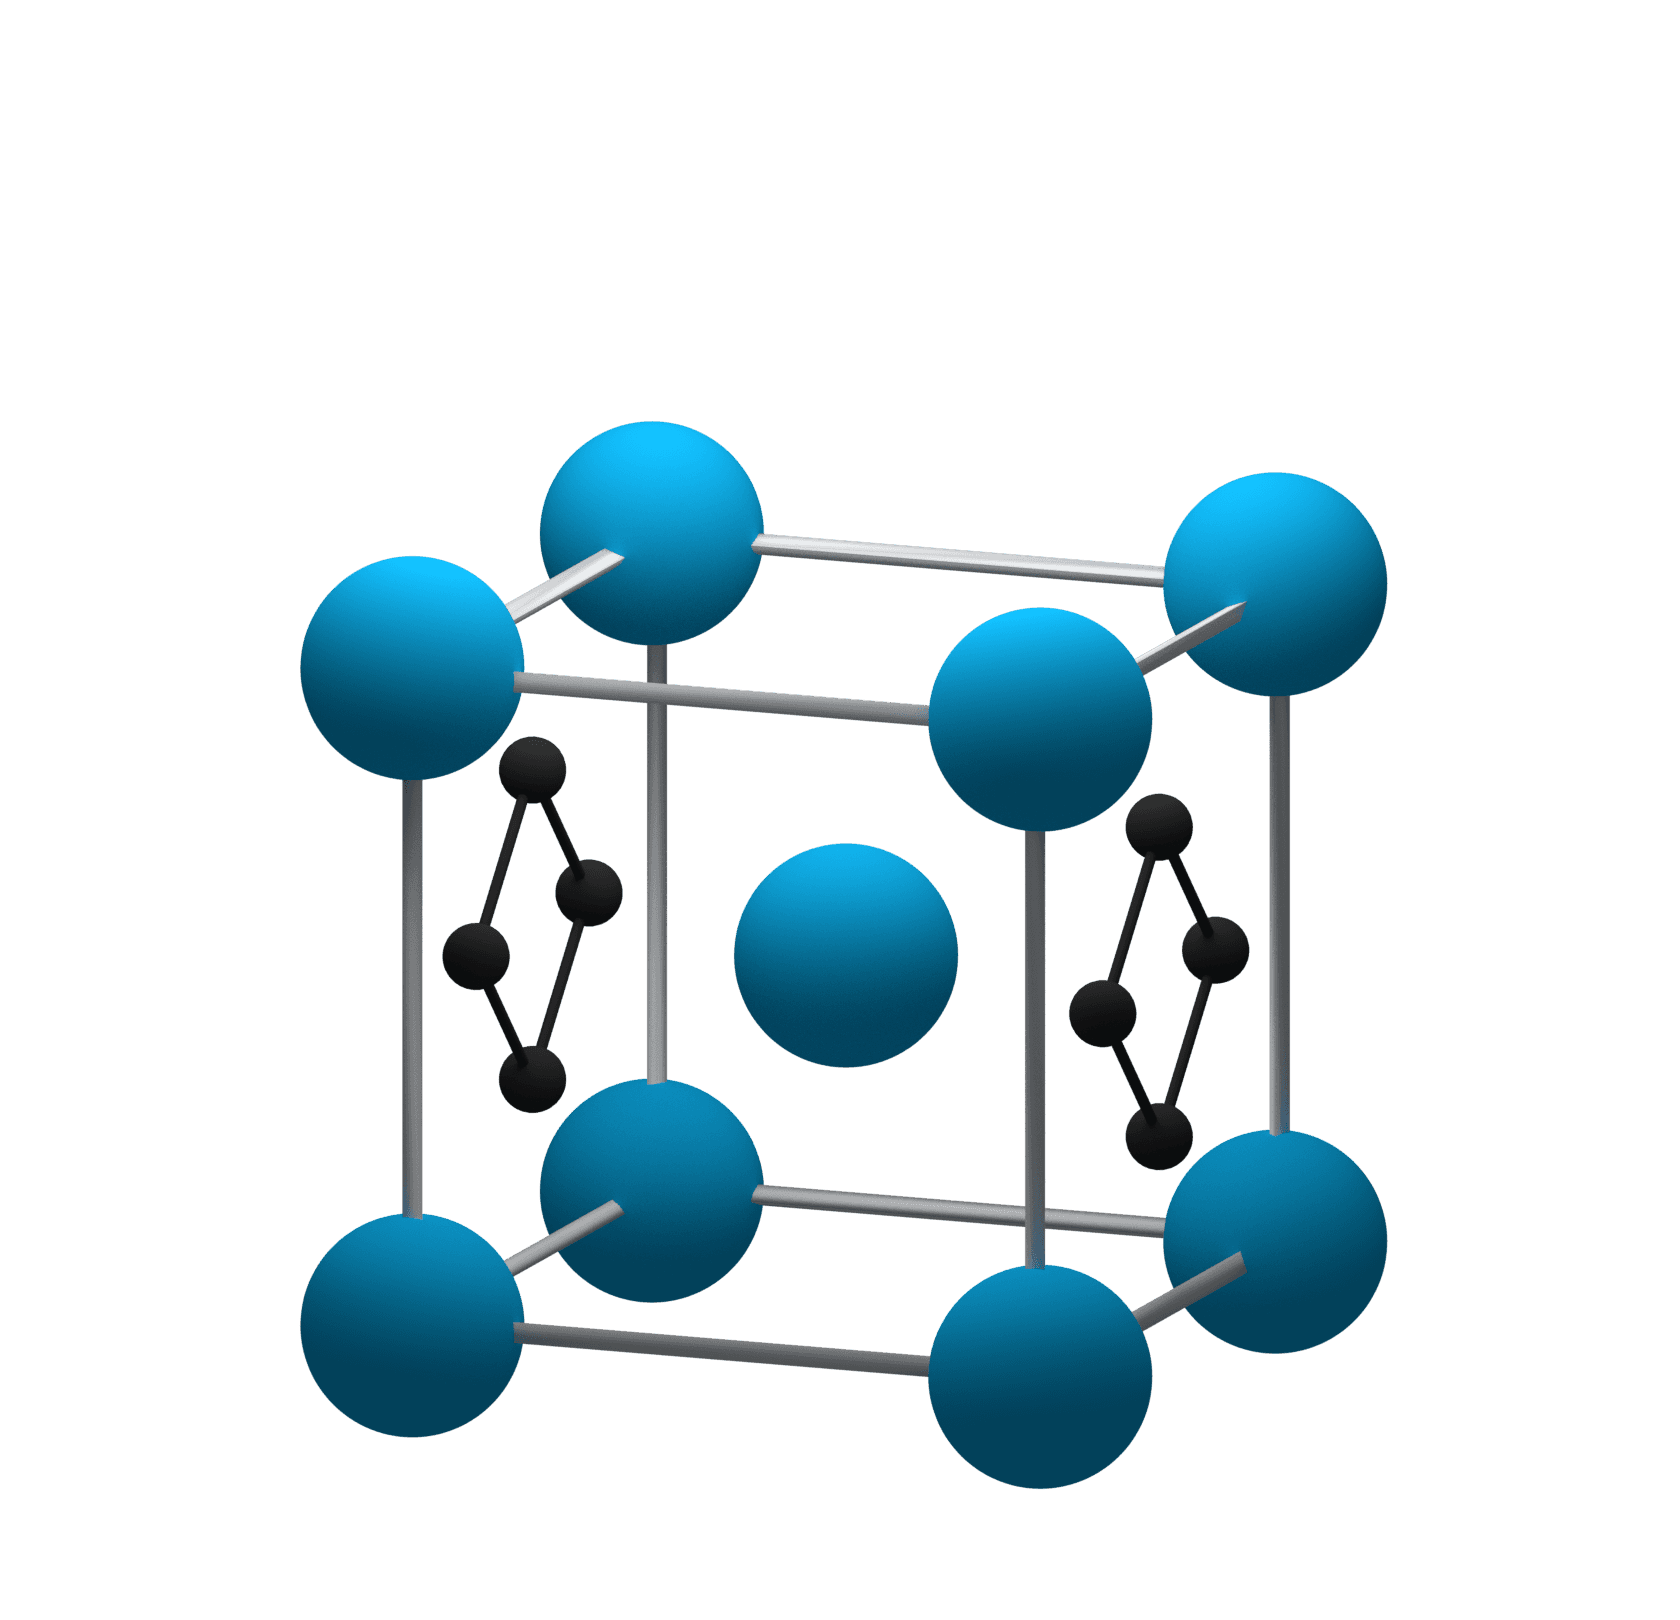
\includegraphics[width=0.3\linewidth]{bcc_render.png}
\caption{The BCC crystalline structure (atoms in blue). Shown in black are 8 out of 24 tetrahedral interstitial positions around the central atom.}
\label{Fig:bcc}
\end{figure}
In a W-H system, formed, e.g. by placing a tungsten object under a hydrogen atmosphere, H atoms tend to lower the system energy by binding to defects. 
E.g. in the case of a vacancy, the empty lattice site leaves neighbouring W atoms with dangling bonds to which hydrogen can bind, leading to a net decrease in energy.

\begin{figure}[!ht]
\center
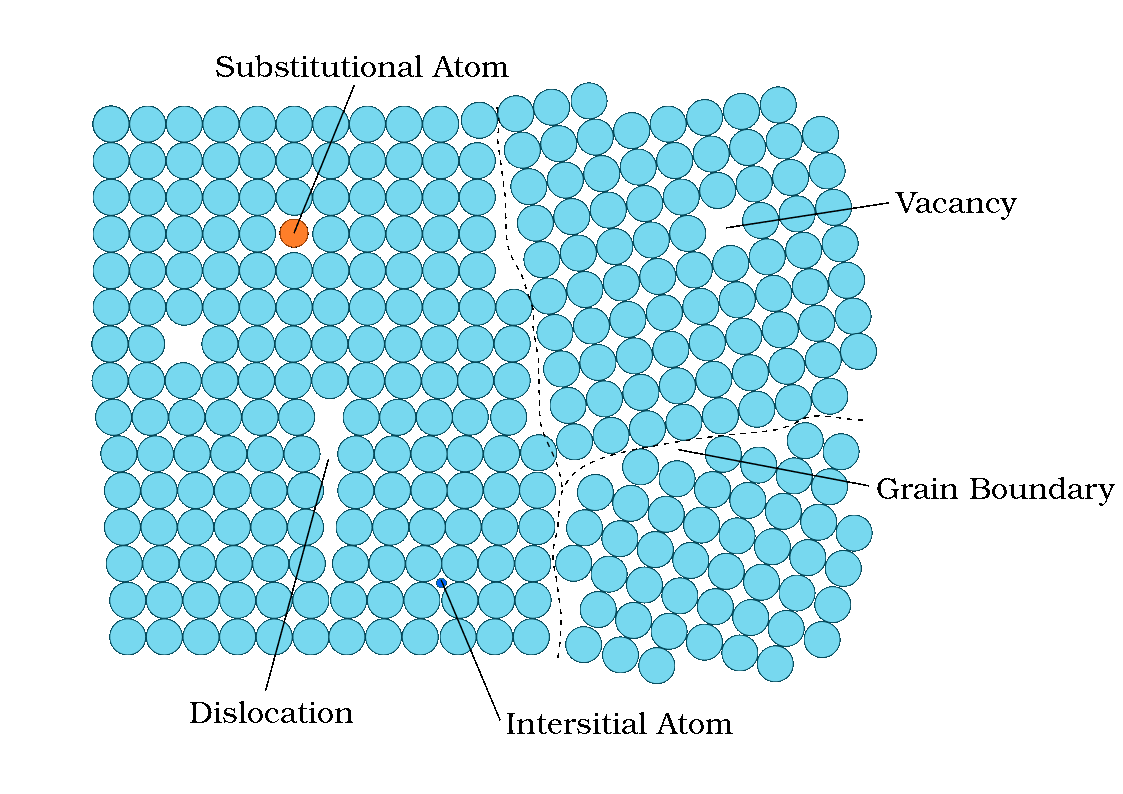
\includegraphics[width=0.76\linewidth]{defect_types.png}
\caption{Various types of crystal defects shown on a 2D lattice}
\label{Fig:defect_types}
\end{figure}


% ---------------------------------------------------------------------------------------------------
\section{Hydrogen Isotope Exchange}
% ---------------------------------------------------------------------------------------------------

The isotopes of a chemical element are essentially variations of the same element, differing in the number of neutrons and thus also atomic mass. 
Since all isotopes of a specific element share the same number of protons and electrons, they can be considered chemically indistinguishable. 
The difference in atomic mass can, nonetheless, present itself as a change in the reaction rates of chemical and thermodynamic processes when an atom is replaced by its isotope. 
Known as the \textit{kinetic isotope effect}, this involves lighter isotopes generally reacting faster than their heavier counterparts. \cite{atkins2006atkins}

In the case of hydrogen, there are three naturally occurring isotopes, protium (H), deuterium (D) and tritium (T). 
In contrast to most other elements, the relative differences in mass between these three isotopes are notably extreme; D ($m_{\text{D}}=2.014102$ u) and T ($m_{\text{T}}=3.016049$ u) have masses of just over two and three times that of H ($m_{\text{H}}=1.007825$ u). 
These mass differences result in, e.g. the isotopes having noticeably different diffusion rates.